% Template for ISBI-2012 paper; to be used with:
%          spconf.sty  - ICASSP/ICIP LaTeX style file, and
%          IEEEbib.bst - IEEE bibliography style file.
% --------------------------------------------------------------------------
\documentclass{article}
\usepackage{spconf,amsmath,graphicx}
\usepackage{amssymb}

%% % For algorithms
%% \usepackage{algorithm}
%% \usepackage{algorithmic}

%% % For text color
%% \usepackage{color}
%% \usepackage{multirow}
%% \usepackage{tabu}

% for table
\usepackage{multirow}

\renewcommand{\vec}[1]{\boldsymbol{#1}}
\newcommand{\mat}[1]{\text{\bf #1}}

% Title.
% ------
%% \title{4D Active cut: a guided interactive tool for pathological anatomy modeling}
%% \title{Traumatic Brain Image Segmentation: An Active Learning Approach}
\title{4D Active Cut: An Interactive Tool for Pathological Anatomy Modeling}
%
% Single address.
% ---------------
\name{Bo Wang$^{\dag,\ddag}$, Wei Liu$^{\dag,\ddag}$, Marcel
  Prastawa$^{\dag,\ddag}$, Andrei Irimia$^{\S}$, \vspace*{-1.5ex}}

\nameLots{Paul M. Vespa$^{\natural}$, John D. van Horn$^{\S}$, P. Thomas
  Fletcher$^{\dag,\ddag}$, Guido Gerig$^{\dag,\ddag}$\vspace*{-1ex}\sthanks{
    Supported by grants: National Alliance for Medical Image Computing (NA-MIC)
    U54 EB005149 (GG) and the Utah Science Technology and Research (USTAR)
    initiative at the University of Utah.  }}
%This work is part of the National Alliance for Medical Image Computing (NAMIC),
%funded by the National Institutes of Health through the NIH %Roadmap for
%Medical Research, Grant U54 EB005149.

\address{
\begin{tabular}{cc}
$^{\dag}$ Scientific Computing and Imaging Institute, &
$^{\S}$ Institute for Neuroimaging and Informatics, USC \\
$^{\ddag}$ School of Computing, University of Utah & $^{\natural}$ Brain Injury Research Center, UCLA
\end{tabular}
}

\begin{document}

%
\maketitle
%
\begin{abstract}
4D pathological anatomy modeling is key to understanding complex
pathological brain images. It is a challenging problem due to the difficulties
in detecting multiple appearing and disappearing lesions across time points and estimating
dynamic changes and deformations between them.
We propose a novel semi-supervised method, called \emph{4D active cut}
for lesion recognition and deformation estimation. Existing
interactive segmentation methods passively waits for user to refine the
segmentations which is a difficult task in 3D images that change over time.
\emph{4D active cut} instead
actively selects candidate regions for querying the user, and therefore
obtains the most informative user feedback. A user simply answers `yes' or `no' to
a candidate object without having to refine the segmentation slice by
slice. Compared to single-object detection of GrabCut, our method also
detects multiple lesions with spatial coherence using Markov random
fields constraints. Results show improvement on the lesion detection, which
subsequently improves deformation estimation.
\end{abstract}
%
\begin{keywords}
Active learning, graph cuts, longitudinal MRI, Markov Random Fields,
semi-supervised learning, \end{keywords}
%

\section{Introduction}
\label{sec:intro}

Quantitative studies in longitudinal pathology such as traumatic brain injury
(TBI), autism, and Huntington's disease are important for
measuring treatment efficacy or making predictions. The
modeling of 4D pathological anatomy is essential to understand the complex
dynamics of pathologies and enables other analysis such as structural pathology and
brain connectivity \cite{Irimia2012}. This is a challenging task because of the
difficulties in localizing multiple lesions at specific time points and
estimating deformations between time points. In effect, this involves
solving interdependent segmentation and registration problems.
In the analysis of magnetic resonance (MR) images of severe TBI patients,
more difficulties arise such as multiple lesions with complex shapes,
multi-modal information, and lack of prior knowledge of lesion
location.
%The state-of-art image segmentation algorithms often fail to find the
%true lesions, with high false-positive rate for single lesion detection, and
%high false-negative rate in multiple lesion detection.

%However, for TBI images, a standalone algorithm
%such as graph cuts could not achieve good results without a human expert's
%involvement.
%We note a little user input at the right time and right place can
%significantly improve the algorithm's performance.
Graph cuts based user-interactive image segmentation methods have been applied
to 2D and 3D imaging data \cite{boykov2001fast,rother2004grabcut}.  In
particular, the GrabCut method~\cite{rother2004grabcut} integrates human experts'
knowledge and the algorithm's computation power. In GrabCut, one typically gives
an initial guess of the region of interest (foreground), for example a bounding
box. The algorithm estimates globally optimal boundary between the foreground
and background regions. The user then inspects the segmentation results, and
adjusts the boundary by drawing a region as a hard constraint. Such process
works well on 2D images, as users can quickly find incorrectly classified
regions. However, such interaction is a huge burden to users once applied to 3D
volume data, since one has to visually inspect each slice and correct it.  The
algorithm is in a \emph{passive learning} state, and its performance entirely
depends on user's active inspection and correction. This passive learning
process is the bottleneck of the GrabCut algorithm when applied to 3D data.

% existing algorithm's issue: large false positive.

% Motivate our methods. active learning, multiple objects, MRF prior, query
% score, low false positive, low user interaction workload. Global optimum
% (graphcuts).

We propose \emph{4D active cut}, a method that uses active learning
for guiding interactive segmentation of 4D pathological images,
specifically longitudinal TBI data.
We adopt a minimalist approach such that our
algorithm needs the least amount of user involvement.
Using active learning, the algorithm queries the user only on the most
important regions. Accordingly,
the user's response to such query will be the most informative, and the number
of user interaction is minimized. Our algorithm learns the model from a simple
user initialization, finds the candidate objects and submits them to a user for
inspection. The user is now in a passive state, and are only required
to answer a `yes' or `no' question for the queried candidates.
The algorithm does the remaining work
including refining the candidate objects, learning model parameters and running
graph cut algorithm to find a globally optimal map. In addition, with sufficient
confidence, the algorithm automatically identifies additional lesion objects
without user interaction by self-training. Self-training further decreases
user involvement, without losing segmentation accuracy.
Our algorithm can detect multiple lesions, while standard graph
cut algorithm~\cite{rother2004grabcut} only detects single objects. Moreover, we
introduce spatial context constraints using Markov random fields (MRF) so
that the estimated label maps will become piecewise constant.
We also define the MRF prior on the candidate objects submitted to the
user, so the candidates are spatially coherent objects instead of individual
 voxels.

%% Besides the energy term of the graph cut's objective function to get smooth
%% boundary between normal and lesion regions, we also define a MRF prior on label
%% variables within the normal and abnormal class.

Several researchers have applied active learning to 3D image segmentation.  Top
et al.~\cite{top2011active} proposed to query users the most uncertain 2D slices.
Iglesias et al.~\cite{iglesias2011combining} used active learning for
constructing manually labeled dataset for training supervised classifiers.
Veeraraghavan et al.~\cite{veeraraghavan2011active} used grow cut for
segmentation and estimated the uncertainty using a support vector machine
classifier. Our method is different from them in that 1) it solves  both
segmentation and registration in a unified 4D framework, and 2) instead of learning 2D
slices or individual voxels, it learns new 3D objects that better fit human
visual perception due to their spatial coherence.


%% above ones since it is a 4D framework solving both segmentation
%% and registration problems. In addition, our algorithm differs in that instead of
%% learning new voxels, it learns new objects that better fit human visual
%% perception due to their spatial coherence.

In the remaining part of the paper, we discuss the model and interaction
framework in section \ref{sec:method}, give the 4D modeling results in section
\ref{sec:results} and conclude in section \ref{sec:conc}.


%% algorithm in
%% which segmentation is performed by grow cut and uncertainty of segmentation is
%% estimated by support vector machine to give suggestion to user. The drawbacks of
%% this method are: the segmentation and uncertainty estimation are separated, the
%% algorithm is for single object segmentation, and the suggestion for user are
%% pixels which are not informative and not compact.  We propose a new objective
%% function for both graph cuts segmentation and uncertainty estimation for active
%% learning which naturally put both components into one unified framework.

\section{Method}
\label{sec:method}

%% An overview of our framework is shown in Fig. \ref{fig:flowchart}. At one time point, the algorithm is initialized by a bounding box given by user which is converted to hard constraint. Mixture of Gaussian (GMM) and Graph Cuts are used to perform probabilistic segmentation. Given the result of GMM and Graph Cuts, query score is computed to decide if self-training (ST) or active learning (AL) should be executed. After this, either ST or AL is performed, so the hard constraint is updated. Using the new hard constraint, the algorithm runs the next iteration of segmentation and user interaction until it is stopped by user.
%% After repeating above process for each time point, 4D modeling is performed which is the end of 4D active cut.
An overview of our algorithm is shown in Fig.~\ref{fig:flowchart}.
At each time point, the algorithm takes a bounding box as the initial
user input, learns the model parameters, estimates graph cuts for detecting
the lesions, and queries a user by submitting one or more candidate objects.
The 3D label information from all time points are then integrated
by fitting a 4D model that describes the changes across time as deformations.

\subsection{Extension to GrabCut}
We extend GrabCut~\cite{boykov2001fast,rother2004grabcut} to include
hierarchical smoothness constraints. We build two GMM models for the normal
brain regions and the lesions, and use the expectation maximization (EM) method
to estimate both the class labels and the model parameters $\theta$. In the
graph cut step, the algorithm takes model parameters of both GMMs as input, and
estimates a hard label $\alpha \in \{0, 1\}$ representing if each voxel $n$ is
normal ($\alpha_n =0 $) or lesions ($\alpha_n = 1$). In addition to smoothness
constraint on the lesion boundary, we also apply MRF constraints on the label
maps within normal and lesion regions. These soft constraints guarantee that
the estimated labels are spatially coherent.

\noindent \textbf{Within-Class MRF and Variational Inference}: Define the class
label map $\mat z = \{\vec z_1, \dots, \vec z_N\}$, where $\vec z_n$ is a K
dimensional binary random variable for voxel $n$ such that $\sum_k \!z_{nk}
\!=\! 1$. An element $z_{nk}\!=\!1$ indicates voxel $n$ is in Gaussian component
$k$. The prior distribution of $\mat z$ takes the MRF constraints into account
as well as the atlas, and is defined as
\begin{equation*}
  p(\mat z) = \frac{1}{C} \exp( \sum_{n=1}^N \sum_{k=1}^K z_{nk} \log \pi_{nk} + \beta \!\!\sum_{(n,m)} \langle \vec z_n, \vec z_m \rangle ),
\end{equation*}
where $\pi_{nk}$ is the affine-registered atlas prior probability of $n$ being
in component $k$, $(n, m)$ is a pair of neighboring voxels, and $\langle, \rangle$
is the inner product of two vectors, representing our preference of a piecewise
constant label map, with the constraint strength given by $\beta$. Given $\vec
z_n$, the likelihood function is defined as a multivariate Gaussian $p(\vec x_n |
\vec z_n) = \mathcal{N}(\vec x_n; \theta(\vec z_n))$, with $\vec x_n$ being the
observed data vector of the multi-modality images at $n$. In EM, one needs to
evaluate $\mathbb{E}_{P(\mat z |\mat x)} [\log p(\mat x, \mat z)]$, which is
intractable due to the MRF prior on $\mat z$. Here we use the variational
inference method that iteratively updates $p(\vec z_n|\vec z_{\mathcal{N}(n)},
\vec x_n)$ given the expected value of $\vec z_n$'s neighbors
$\mathcal{N}(n)$. The update equation takes the form
\begin{equation*}
  \log p(z_{nk}) = z_{nk} \pi_{nk} + \!\!\!\!\! \sum_{m\in \mathcal{N}(n)} \!\!\!\langle \overline {\vec z}_m, \vec z_n \rangle + \log \mathcal{N} (\vec x_n; \theta(\vec z_n)),
\end{equation*}
where $\overline {\vec z}_m$ is the expected value at neighbor $m$. We
compute $\log p(z_{nk})$ for all $k$ and compute $p(\vec z_n)$ by taking the
exponential and normalize. $\overline{z}_n$ is just $p(\vec z_n)$ for binary
variables and is used for updating $\vec z_n$'s neighbors. In the M step, we
use $\mat z$ to estimate $\theta = \{\mu, \Sigma\}$ for all components. The
variational procedure stops when there are no changes of $\vec z_n$. Given $\alpha$, EM runs
on both GMMs separately, with a uniform atlas map on lesion's GMM.

\begin{figure} [t]
\centering
%% 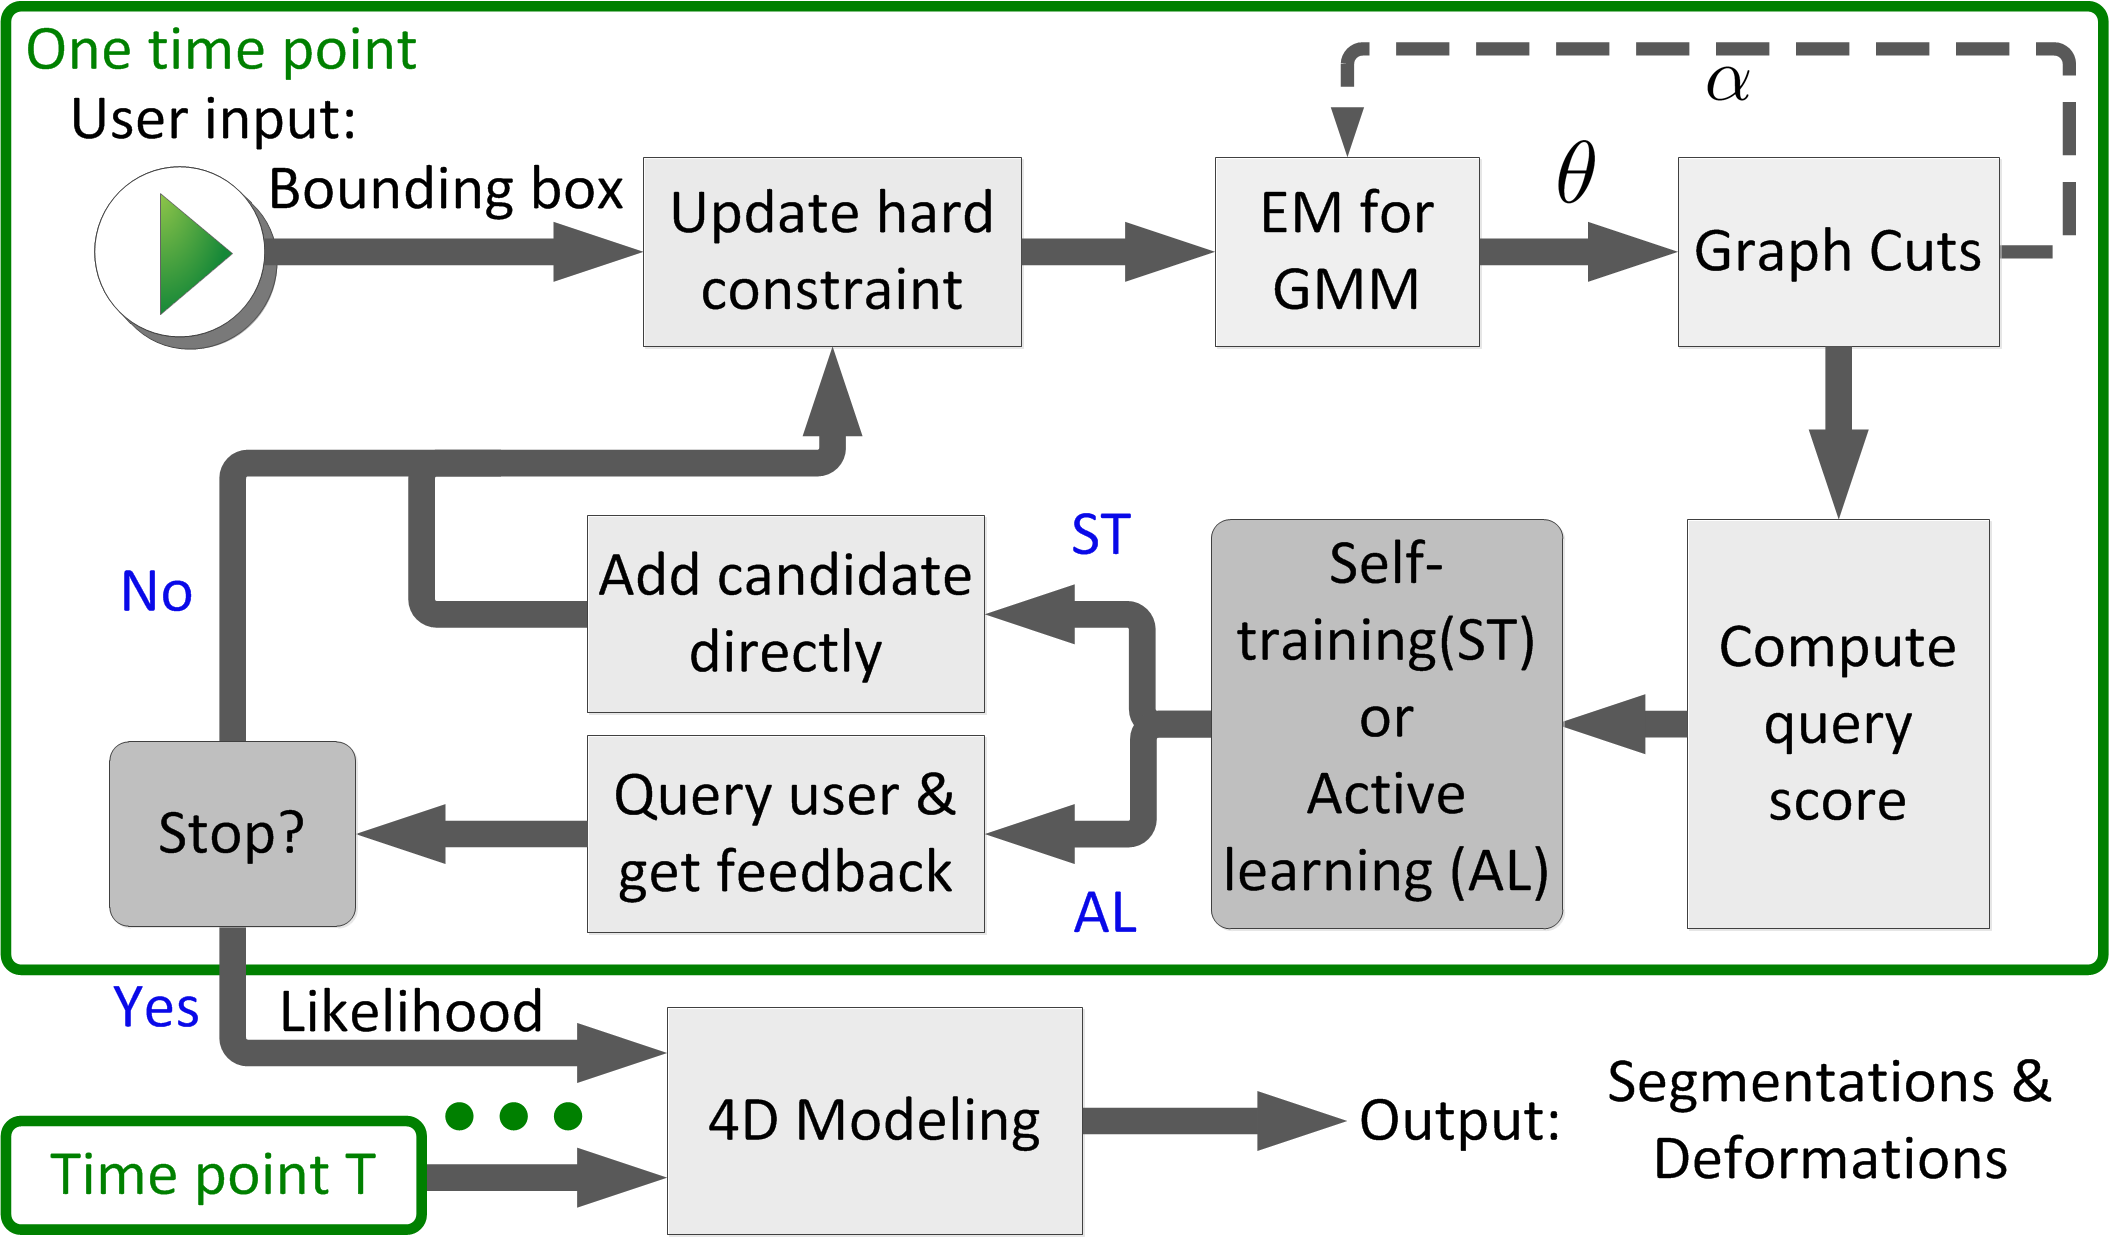
\includegraphics[width=8.5cm]{./figures/acLearn_flowchart}
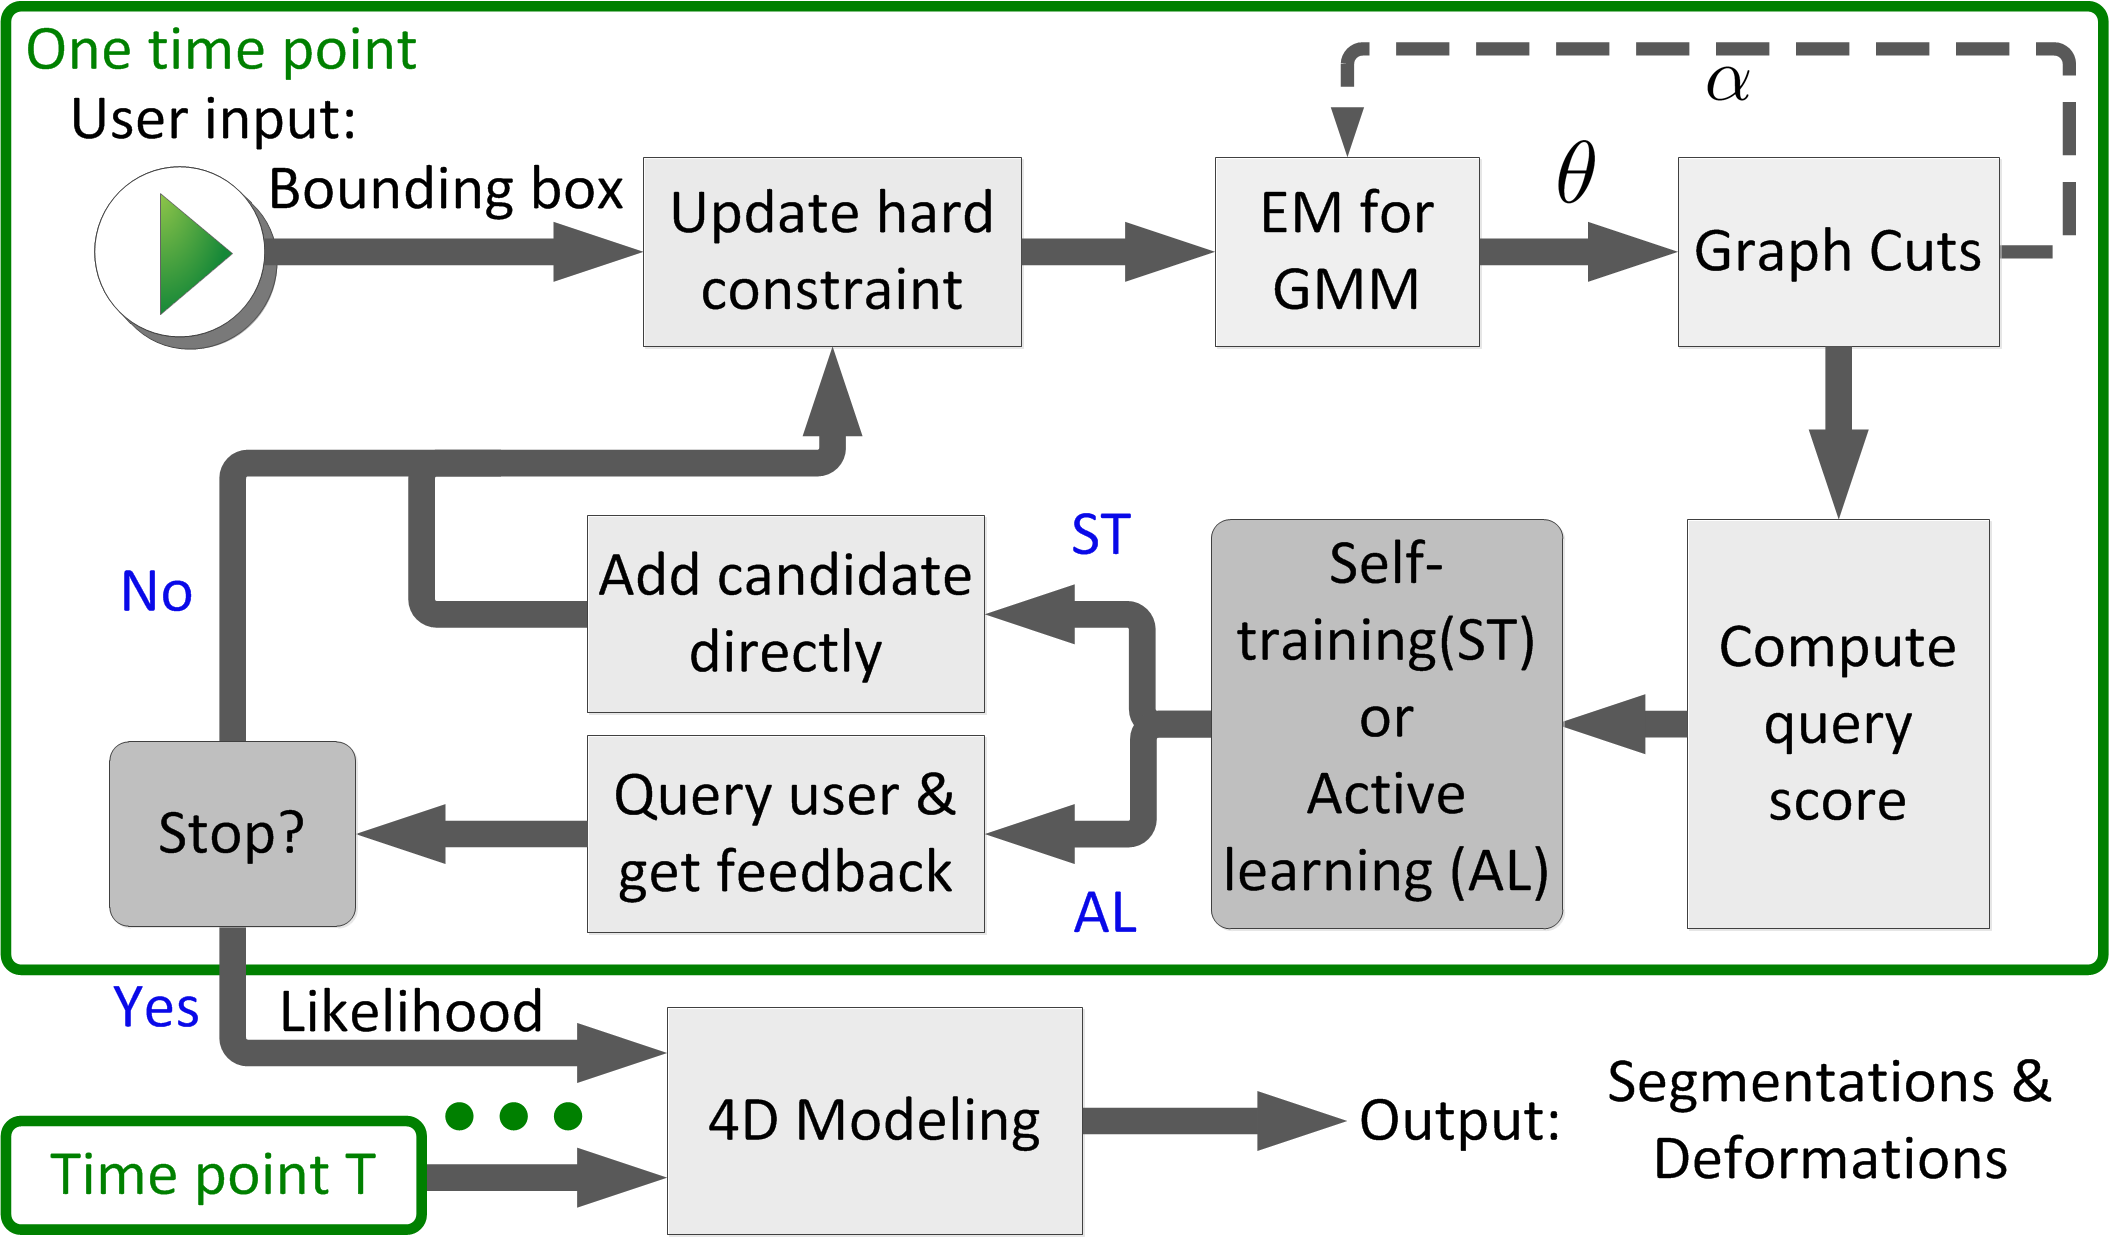
\includegraphics[width=0.479\textwidth]{./figures/acLearn_flowchart}
\caption{Flowchart of the proposed algorithm.}
\label{fig:flowchart}
\end{figure}
%-------------------------------------------------------------------------
%\subsection{Active Learning New Object}
%\subsection{Active-cut based 4D Pathological Anatomy Modeling}
\subsection{Guided User Interaction Using Active Learning}

% Gives a short intro of active learning with (just one) reference. Why active
% learning, benefit. How that works in general. Then talk about our
% strategy. Need to mention self-training (automatically add unlabeled data into
% labeled dataset, thus decreasing user interaction/burden).

The algorithm conducts active learning by taking $\alpha$ and $\theta$ as
input, and computing the probability of each voxel belonging to the lesions. It
then builds a connected component map, since a high-level object-based
representation is convenient for user interaction. We sort the multiple objects
in a descending order of the probability of being lesions, and submit the
top ranked objects for queries to the user.
When the algorithm detects that the top ranked object should
be lesion with a confidence above a user-given threshold, it adds the object
to lesion in a self-training process without querying users, further
reducing user involvement.

% How the query score are computed. (LW will add stuff here)
\noindent\textbf{Query Score: }The log-odds of $\alpha_n$ is defined as
\begin{align*}
  a_n = \log p(\alpha_n=1) + \mathbb{E}_{p(\vec z_n|\vec x_n)} [\log p(\vec x_n, \vec z_n; \theta (\alpha_n=1))]\\
  - \log p(\alpha_n=0) + \mathbb{E}_{p(\vec z_n|\vec x_n)} [\log p(\vec x_n, \vec z_n; \theta (\alpha_n=0))],
\end{align*}
where $\mathbb{E}$ is the expectation, $\alpha$ is a MRF in the form of
$p(\alpha) = (1/C_{\alpha})\exp (\eta \sum_{(\alpha_m, \alpha_n)} \psi(\alpha_m,
\alpha_n ) )$ to model its spatial coherence, with $\psi =1$ if $\alpha_m =
\alpha_n$, and $\psi = 0$ otherwise. The predictive probability of a voxel being
in lesion is computed by the standard logistic function $p(\alpha_n=1|\vec x_n)
= 1/ (1 + \exp (-a_n))$ once $a$ is estimated by the variational inference. We
obtain a binary map $\vec w$ by thresholding the predictive map at 0.5, and
identify a series of objects $R_i$ by running a connected component detection on
$\vec w$. To further select the most salient objects, we sort the objects in
decending order of the following score:
\begin{align}
q(R_i) = \left (\sum_{n\in R_i} p(\alpha = 1| \vec x_n)  \right ) \Big /  \vert\{n: n\in \mathcal{B}(R_i) \}\vert.
\label{eq:score}
\end{align}
$\mathcal{B}(R_i)$ is the set of voxels on $R_i$'s boundary, and the denominator
denotes the number of voxels on the boundary of $R_i$. The above query score
prefers objects with larger volumes of posterior probability. The score also
prefers blob-like objects since such an object has large volume-surface
ratio. Such criteria reflects our prior knowledge on the lesion object's shape.

% parameters empirically chosen, but not have big impact on results. Need to say
% that!

\noindent\textbf{4D Modeling Pathological Anatomy: }
We integrate the 3D information across time by taking $\mat z$ and $\theta$ for
both normal and lesion classes as input, and estimate the atlas prior $\pi$ by
computing the deformation from the healthy template to the images at each time
point. We follow the 4D pathological anatomy modeling framework of Wang et
al. \cite{WangMBIA2013}, and define $\pi_{k,t} = A_k \circ \phi_t + Q_{k,t}$,
where $A$ is the tissue class probability that is initially associated with the
healthy template, $\phi_t$ is the diffeomorphic deformation from time $t$ to the
atlas, and $Q_t$ is the non-diffeomorphic probabilistic change. We use alternating
gradient descent to estimate $A$, $\phi_t$ and $Q_t$ by optimizing
$\mathcal{F}(A, \phi_t, Q_t) = - \sum_{t=1}^T \mathbb{E}_{p(\mat z| \mat
  x)}[\log p (\mat z, \mat x| \theta, \pi_t)]$.

% Give a summary of the pipeline. and give reference of pipeline's figure.
\noindent\textbf{Interaction Framework: } With the above framework, the
learning process is described in Fig. \ref{fig:flowchart}. Given the user defined
bounding box, the hard-constrain map is set to `normal' outside the box, and
`uncertain' inside. Then, we initialize the $\alpha$ map such that $\alpha \!=
\!1$ (lesion) in the `uncertain' region of the hard-constrain, and $\alpha \!=
\!0$ elsewhere. The EM learns $\theta$ of both GMMs given $\alpha$, then a
graph-cut step~\cite{rother2004grabcut} updates only the $\alpha$ for voxels
within the `uncertain' region. This update strategy of graph-cuts prevents
false-positive detections. Upon EM \& graph cuts convergence, there may be some
false-negative voxels in `normal' regions. We group these voxels into spatially
coherent objects and find the one with highest score computed from
\eqref{eq:score}. The algorithm either automatically adds the candidate to
lesions or queries user for answer, depending on its confidence on the
candidate. We then update the hard-constraint map to reflect the knowledge
learned from the new object, and a new EM \& graph cuts iteration starts.
Objects already accepted or rejected in previous steps are recorded so they will
be excluded from future queries. This learning process repeats until
user stops the algorithm. Finally, we integrate information in the
longitudinal datasets in all time points by fitting a 4D pathological anatomy
model.

\section{Results}
\label{sec:results}
We applied our method to a dataset of longitudinal multimodal MR images of four
severe TBI patients.  Each patient was scanned twice: an acute scan at about 5
days and a chronic scan at about 6 months post injury. Each subject's data
includes T1, T2, FLAIR, and GRE. In lesions' GMM model, we chose $K=2$ for
bleeding and edema component, and in normal regions we chose $K=3$ for gray
matter, white matter and CSF. We took a 6 neighborhood system and set the
smoothness parameters $\gamma = \beta = \eta = 1$. The image intensity of each
modality was normalized to the range [0, 255] before the learning process. We
used the K-Means clustering together with the atlas prior to initialize the
GMM. The threshold used to decide self-training or active-learning was set to
3.0.

\begin{figure} [ht]
\centering
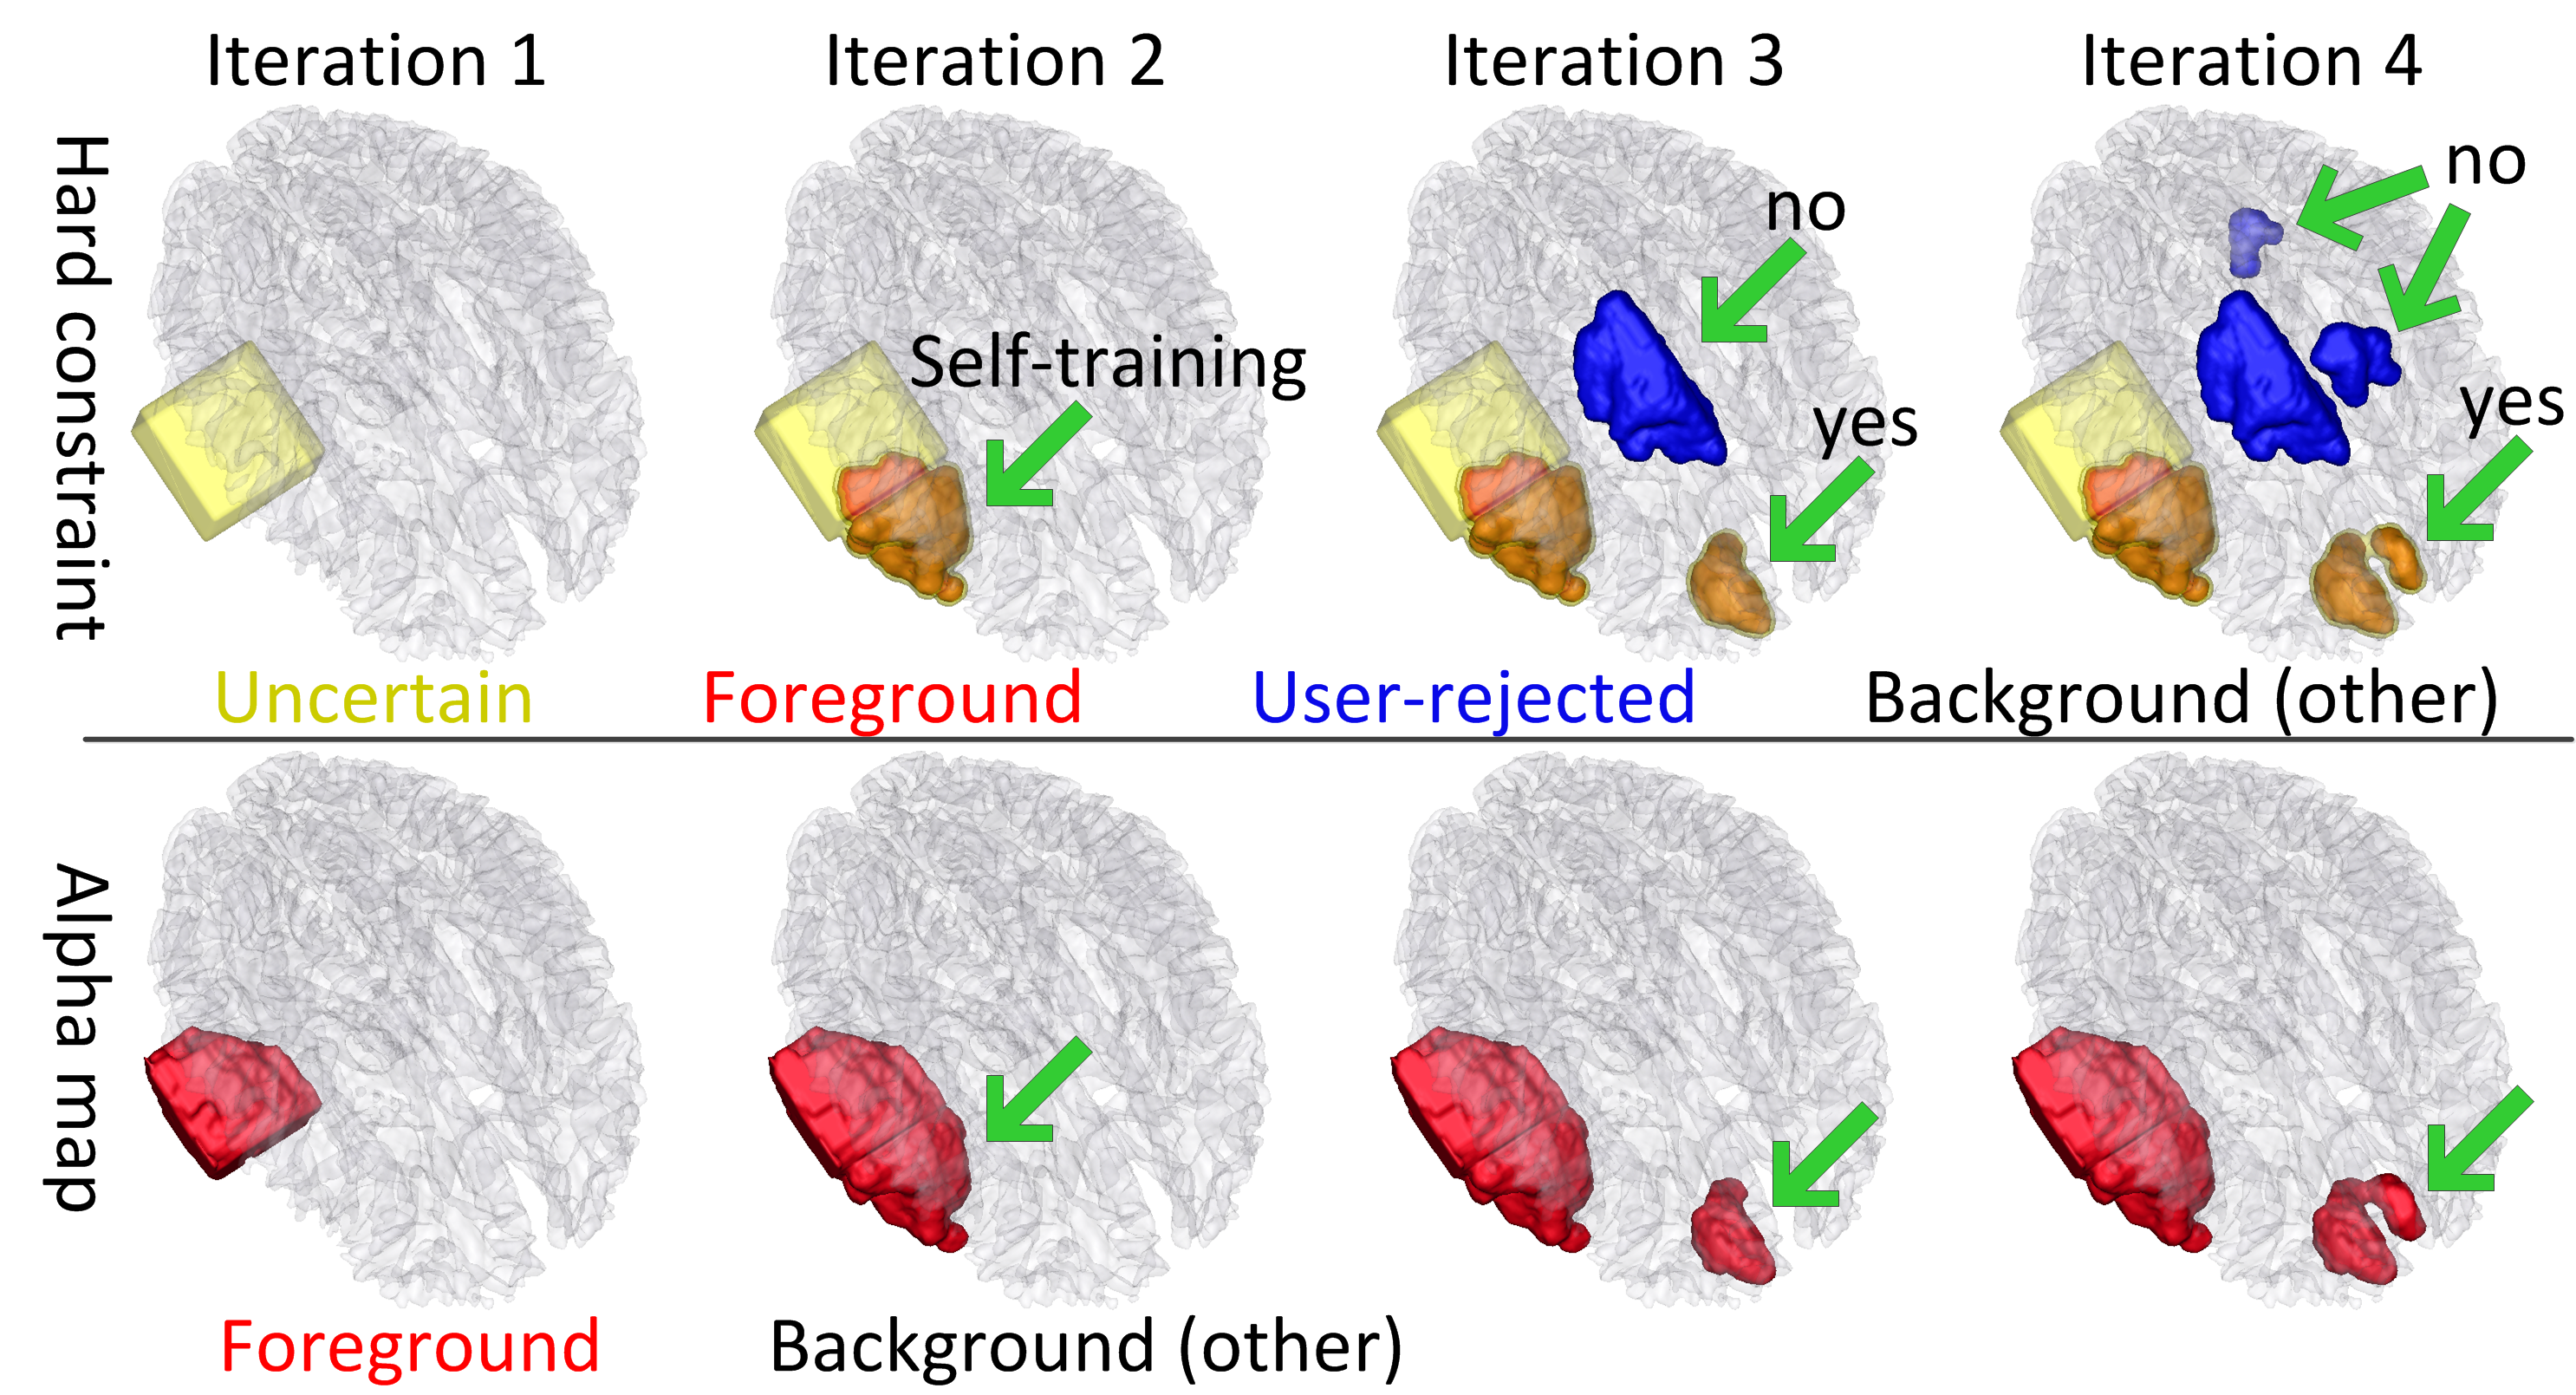
\includegraphics[width=0.479\textwidth]{./figures/iterative_process_new}
\caption{Illustration of the iterative process of 4D active cut on subject
  I. Iteration 1: User-initialized bounding box. Iteration 2: Self
  training. Iteration 3 and 4: Active learning. The user stopped the process at 5th
  iteration. Arrows point to the changes between iterations. The white matter
  surface is visualized in all figures as reference.
}
\label{fig:userinter}
\end{figure}

Fig.~\ref{fig:userinter} shows the dynamic learning process of subject I. In
iteration 1, given the user initialized bounding box, 4D active cut successfully
detected the lesion object, as shown in the bottom $\alpha$ map. In iteration 2,
the candidate object has a large query score, so the algorithm decided to do
self training and added the candidate to the lesion class. This object is indeed
part of the lesion in the previous bounding box. That shows when the user leaves
a portion of the lesion outside the box, the algorithm still detects the
missing portion. This result shows the robustness of the algorithm given
inaccurate user initialization. In iteration 3 and 4, the user rejected some
candidate objects and accepted some others.  The accepted objects are not
connected to the major lesion but our algorithm still captured them. This result
shows that our method is able to detect multiple objects. We also note that by
using object volume, predictive probability and shape information, most of the
top-ranked candidates are indeed true positive ones; showing the effectiveness
of the proposed query score.

\begin{figure} [ht]
\centering
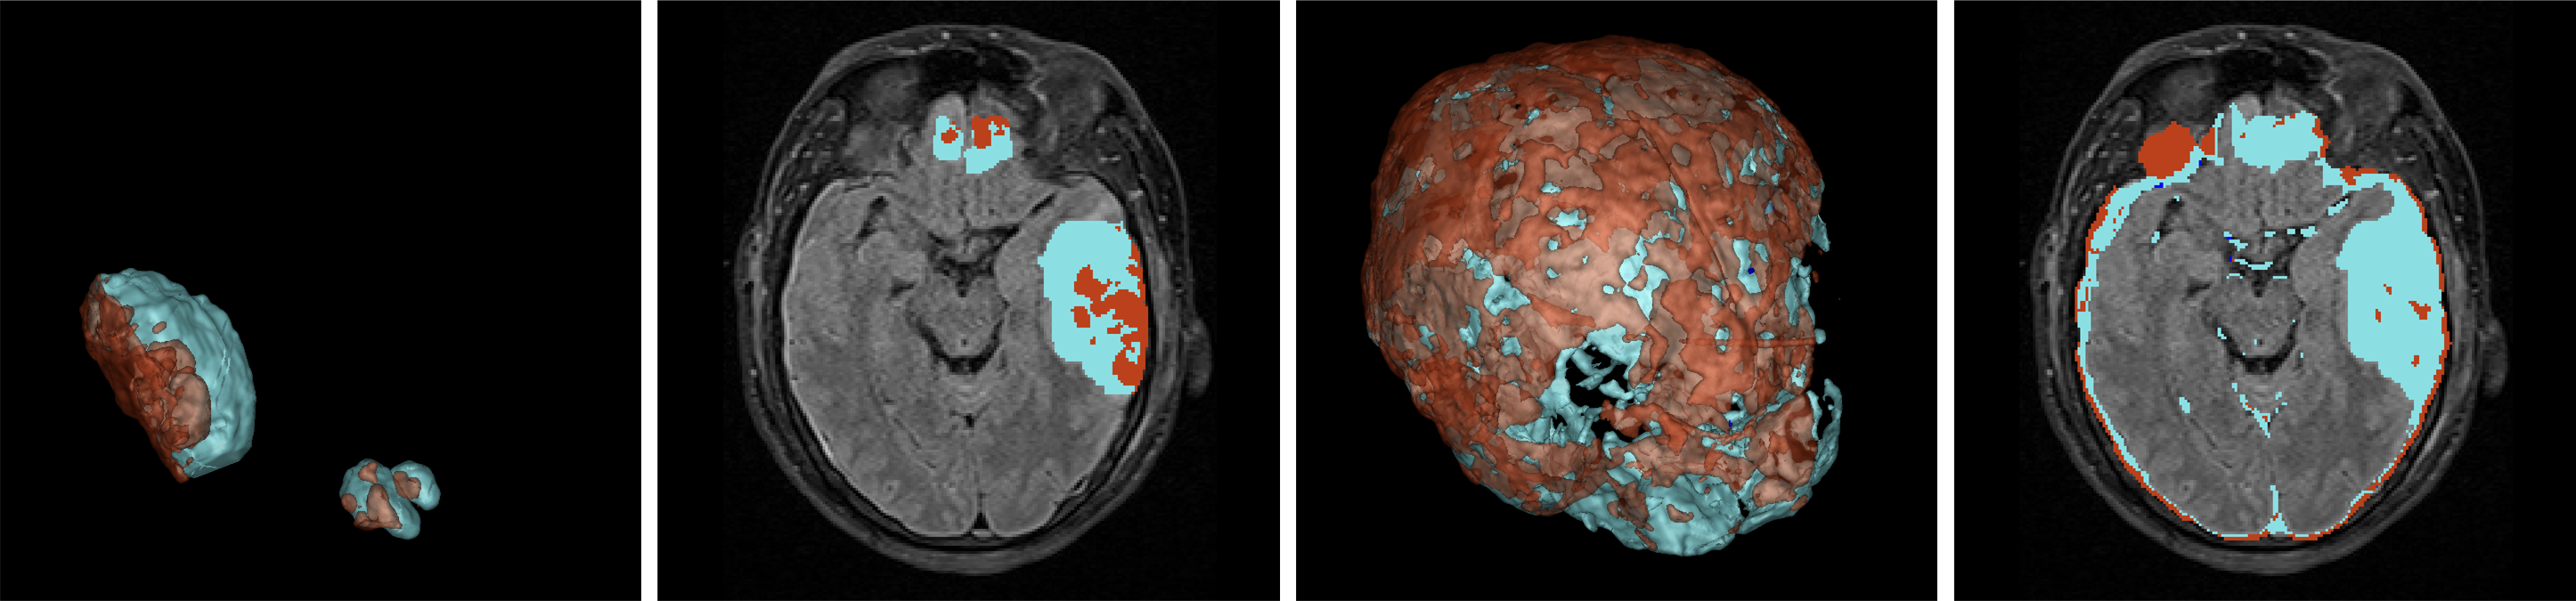
\includegraphics[width=0.479\textwidth]{./figures/qualitative_comp}
\caption{Comparison between GrabCut and the proposed method. Left: our
  method in 3D space and axial view. Right: GrabCut. Light blue: edema. Brown:
  bleeding. Note the large false-positive detection of GrabCut in the CSF
  region.}
\label{fig:QualComp}
\end{figure}

\begin{table} [ht]
%\begin{center}
\centering
\begin{tabular}{c|cc|cc|c}
\hline
 &  \multicolumn{2}{c}{Baseline} &  \multicolumn{3}{|c}{4D active cut}\\
\cline{2-6}
\multirow{1}{*}{Subject}  & NHL & HL & NHL & HL & UI\\

I  & 0.2503 & 0.0613  & 0.6349 & 0.5698 & 5\\ %\hline
II & 0.3269 & -  & 0.6910 & -   & 4 \\ %\hline
III  & 0.1311 & 0.2288   & 0.4512 & 0.4840 & 6 \\ %\hline
IV   & 0.0918 & 0.0998   & 0.3503 & 0.1153 & 5 \\ \hline
\end{tabular}
\caption{ Dice values comparing \emph{4D active cut} and GrabCut to ground
  truth. HL and NHL are acute hemorrhagic and non-hemorrhagic lesions. UI
  denotes the number of interactions a user performed using \emph{4D active cut}.
  Subject II has no ground truth for HL due to the lack of GRE modality.}
\label{tab:DiceResult}
\end{table}

In order to show the efficacy of the proposed method, we used GrabCut
without user interaction as a baseline method and also allowed $\alpha$ outside
of the bounding box to switch labels in order to detect multiple lesion objects.
Fig.~\ref{fig:QualComp} shows the qualitative comparison of the baseline method
and \emph{4D active cut}. Without user interaction, the baseline algorithm detected a
large number of false-positive voxels due to the ambiguity between lesion
and CSF. Table~\ref{tab:DiceResult} shows the quantitative comparison of both
methods. The proposed method is able to significantly improve the
segmentation.

As part of \emph{4D active cut}, we updated the atlas prior using a 4D
modeling
method~\cite{WangMBIA2013}. Fig.~\ref{fig:Deform} shows the parcellation labels
mapped to the space of each time point by using the estimated deformation field.
The result shows the obtained parcellation maps match the data well, even in the
presence of large deformations at different time points.  Therefore, our
integrated framework has the potential of becoming an important processing step for connectivity
analysis of pathological brain with longitudinal data~\cite{Irimia2012}, where
the mapping of parcellation labels to individual time points in the presence of large pathologies presents the biggest obstacle and currently requires tedious manual corrections and masking.


\section{Conclusions}
\label{sec:conc}
We presented \emph{4D active cut} for quantitative modeling of pathological
anatomy. The new algorithm can detect multiple lesion objects with minimal user
input. The MRF prior ensures the spatially coherent label maps within class and
within candidates.  In the future, we will explore integration of active
learning and 4D modeling, as well as the validation and verification on other
image data presenting pathologies.

\begin{figure} [t]
\centering
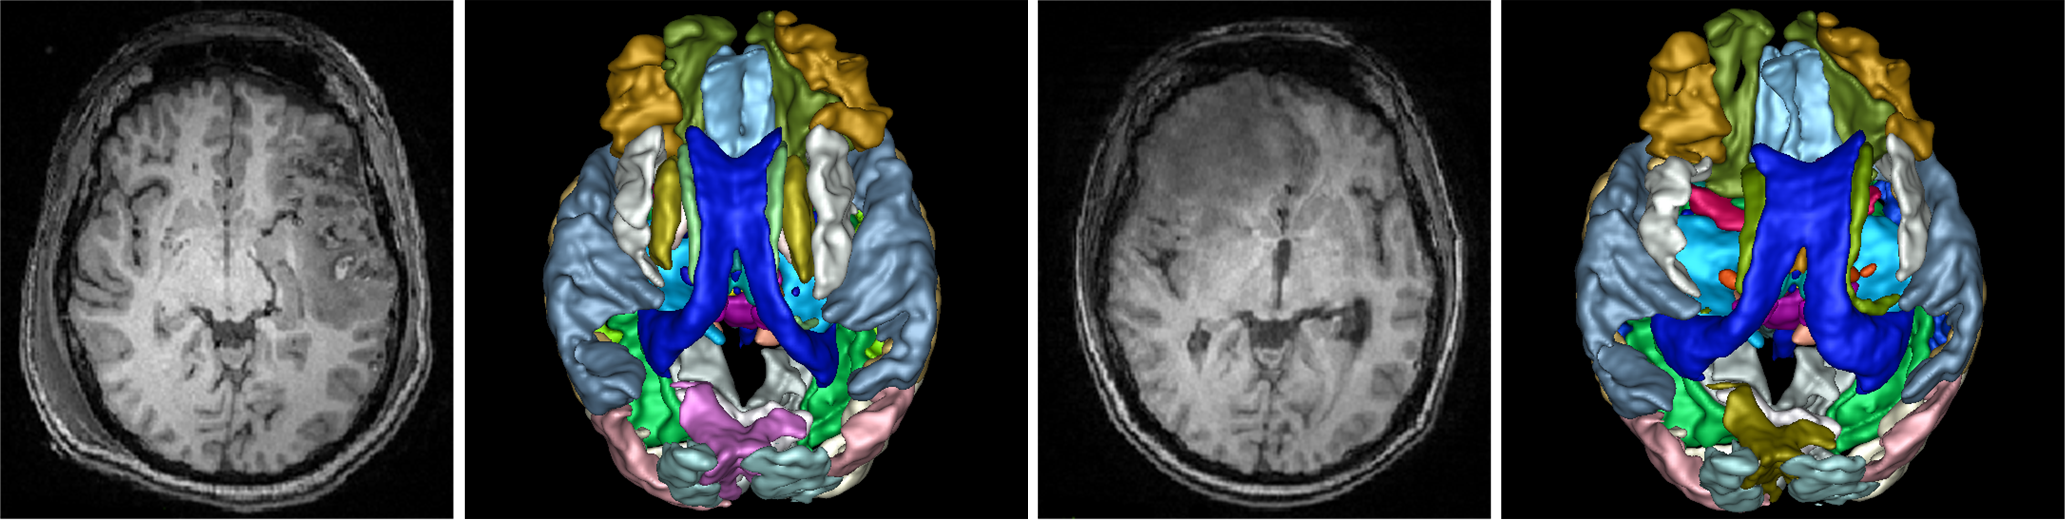
\includegraphics[width=0.479\textwidth]{./figures/parcellation}
\caption{Result of mapping parcellation labels associated with the healthy
  template to each time point. The left two images are the T1 reference TBI image at acute stage and mapped parcellations, and the right two images are the same at chronic stage.}
\label{fig:Deform}
\end{figure}


\bibliographystyle{IEEEbib}
\bibliography{strings,refs}
\end{document}
